\section{Results}
Table \ref{tab:res} contains all of our results that we were able to gather. The graphs \ref{grf:res} and \ref{grf:res2} separate the tested protocols into two sets for readability.
\begin{table}[h]
\begin{center}
    \begin{tabular}{rr|rrrr}
     & \textbf{Size} & \textbf{Alternator} & \textbf{Sequencer} & \textbf{EA Replicator} & \textbf{EAO Sequencer} \\ \hline
    C & 4       & 0.2317443     & 0.21345524    & 0.1863252     & 1.3466524     \\
    Reo & 4     & 0.2843876     & 0.026564892   & 0.03228314    & 0.9987709     \\ \hline
    C & 16      &               & 10.21136      & 0.673219      & 1.831226      \\
    Reo & 16    &               & 1.3540224     & 1.435454      & 3.221851      \\ \hline
    C & 64      &               & 43.723728     & 1.741576      &               \\
    Reo & 64    &               & 34.594992     & 28.79088      &               \\ \hline
    C & 256     &               & 180.61084     & 4.423539      &               \\
    Reo & 256   &               & 254.18812     & 156.3336      &               \\ \hline
    C & 512     &               & 368.2022      & 7.927638      &               \\
    Reo & 512   &               & 761.9697      & 355.2435      &
    \end{tabular}\\
    \caption{All available experiment results}
    \label{tab:res}
\end{center}
\end{table}

\begin{figure}[h]
    \begin{center}
        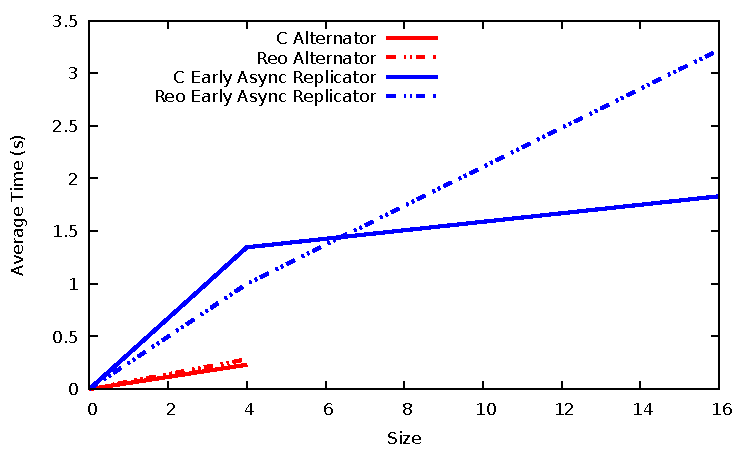
\includegraphics[width=0.7\textwidth]{img/alt-eao.pdf}\\
        \caption{Graph results from the Alternator and Early Async Replicator}
        \label{grf:res}
    \end{center}
\end{figure}
\begin{figure}[h]
    \begin{center}
    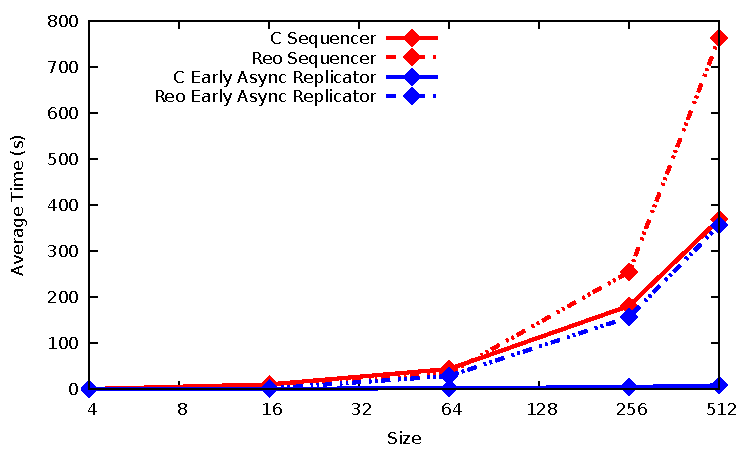
\includegraphics[width=0.7\textwidth]{img/out-seq.pdf}
    \caption{Graph results from the Sequencer and Early Async Replicator}
    \label{grf:res2}
    \end{center}
\end{figure}
